%Vorlage
\documentclass[12pt,a4paper]{scrartcl}
\usepackage[english]{babel} %Für die indirekte Angabe von Umlauten. Es müssen dann Umlaute wie folgt im Code angegeben werden: "a "o "u "s.

\usepackage[utf8]{inputenc}
%Math
\usepackage{amsmath, amsthm, amssymb}
\usepackage{braket}
\newcommand{\tens}[1]{% https://tex.stackexchange.com/questions/171788/always-have-the-ring-of-the-tensor-product-below-the-otimes -> Tensor Product
  \mathbin{\mathop{\otimes}\displaylimits_{#1}}%
}
%Page numbers
\usepackage{enumerate}
%Graphics
\usepackage{graphicx}
\usepackage{array}% http://ctan.org/pkg/array
\usepackage{floatrow}
\graphicspath{{./images/}}
%Quantum circuits http://mirrors.ibiblio.org/CTAN/graphics/pgf/contrib/quantikz/quantikz.pdf
\usepackage{tikz}
\usetikzlibrary{quantikz}
\usepackage{lscape}
\usepackage{setspace}
\onehalfspacing
\usepackage{wrapfig}
\usepackage{hyperref}% für die Einbettung von Hyperlinks
\def\UrlBreaks{\do\/\do-}
\usepackage{multirow}
\usepackage{csquotes} %Quotations
%Code
\usepackage{pythonhighlight}


% Margins
%\usepackage{geometry} % Document Margins
%\setlength{\topmargin}{0cm}
%\setlength{\parindent}{5mm}
%\setlength{\parskip}{2mm}
%\setlength{\evensidemargin}{0mm}
%\setlength{\oddsidemargin}{0cm}
\pagestyle{headings}



\begin{document}
\thispagestyle{empty}
\vspace*{-3cm}
\begin{center}
\large \textsc{Bern University of Applied Sciences}
\vspace{0.5cm}
\hrule
\vspace{4.5cm}
{\Large \textsc{Written Report\\
Bachelor Thesis}}\\
{\large HS 2020/21}\\
\vspace{1cm}
{\Large \bfseries
Generation of synthetic ground truth for ophthalmic medical image analysis}\\

\vspace*{1cm}
{\large Tutor:  Prof. Dr. Tiziano Ronchetti}
\end{center}
\vspace*{1cm}

\begin{abstract}
Machine Learning framework that process ophthalmic OCT images and predicts synthetic vitreal, retinal, choroidal and scleral semantic segmentations based on a combination of Image Augmentation techniques and a Convolutional Neural Network presenting an encoder-decoder structure. After cross-validation the results indicate that our framework can automatically segment a regular OCT scan with a mean Jaccard coeficient of 96,87\%, showcasing a hamming distance of xx\% when compared to human ophthalmologists. Furthermore, the authors describe a detailed workflow involving the utilisation of state of the art machine learning techniques with comprehensive explanations on the data preparation, model implementation and evaluation criteria.  
\end{abstract}

\vspace{2cm}
\hspace*{5.2cm}
\parbox{8.2cm}

\begin{tabular}{ll}

Submitted by: & Emeline Liebeherr\\
& Rayner Zorrilla Alfonzo\\

Submission deadline: & Thursday, June 17th, 2021


\end{tabular}

\newpage
\pagenumbering{Roman}
\tableofcontents

\newpage
\pagenumbering{arabic}
%Und nun kommen wir zur Arbeit und fangen an die Seiten mit Arabischen Zahlen zu zählen

\section{Introduction}\label{s:introduction} 
\subsection{Motivation}
The choroid is one of the layers of the eyeball wall, located between the sclera on the outside and the retina on the inside. The choroid is responsible for the irrigation and circulation of the ocular metabolism in order to supply the outer retina with oxygen and metabolites and is therefore highly vascularised. \cite{choroidExpl}

Its thickness can depend on several factors, including age, blood pressure, anatomic pathologies, etc. It has been found that the thickness of the choroid decreases with age, however several recent research studies on choroidal development during childhood and adolescence contradict this finding. In particular, subfoveal choroidal thickness has been found to be negatively correlated in Asian children, where the prevalence of myopia is higher. Longitudinal studies of adolescents have shown that the eyeball lengthens during the development of myopia. In the case of severe myopia this process is associated with a significant thinning of the choroidal thickness. Therefore the choroidal structure and thickness are strongly considered for monitoring the progression of myopia.\cite{ronchetti2019}

The main challenge in detecting disease progression is to detect even small changes as early as possible. Optical coherence tomography (OCT) imaging allows the capture of highly resolved details of the retina and choroid to detect minute changes in the structure of both membranes.\cite{ronchetti2019}

In order to be able to detect changes in choroidal thickness it is necessary to be able to detect all the different layers of the eyeball wall and their interfaces from OCT scans in order to compare results over several years. 
However, a manual approach raises two important problems: firstly, the number of scans to be processed (layer identification) is considerable \cite{Maloca2019}, secondly, the high vascularity of the choroid makes it difficult to distinguish its border with the sclera \cite{ronchetti2019}.

\subsection{Goal}
The aim of this project is to develop a Deep Learning model capable of processing  ophthalmic  OCT  images  and predicts  synthetic  vitreal,  retinal,  choroidal  and  scleral  semantic  segmentations  based  on  a  combination  of  Image  Augmentation  techniques  and  a Convolutional Neural Network presenting an encoder-decoder structure with a mean Jaccard coefficient of at least 95\%   \cite{Maloca2019}. This will automate the measurements made on the scans and considerably reduce the time needed to produce a result, thus reducing the workload of the experts and ensuring a certain accuracy and standardization in the detection of the choroid. 

\subsection{Contributions}

The contribution of this project lies in the setup and documentation of a software framework capable of generating ground truth images for ophthalmic image medical analysis where the vitreal, retinal, choroidal and scleral compartments are clearly defined. The mentioned framework includes image pre-processing, model implementation and results evaluation. 

\subsection{Material and Methods}

\subsubsection{Methodology}

A Convolutional Neural Network (CNN) was designed based on the U-Net CNN model created by Prof. Dr. O. Ronneberger in 2015 \cite{Ronneberger2015}. Following the general machine learning worklow, we used different techniques of data pre-processing that include vectorization, categorization and augmentation of the annotated images in order to train the network. Hyperparameters were modified both empirically from the result of several training sessions and using best algorithmic practices for weighting and learning rate selection. Finally, the images resulting of the CNN predictions are evaluated by using different metrics commonly tracked on Machine Learning (ML) projects like the Dice and Jacard coeficients, sensitivity, specificity and for evaluating the loss a weighted version of the categorical crossentropy. Statistical Rigurosity??????

\subsubsection{Data}

The OCT B-Scans used in this project are a subset of a total 180 3D OCT volume stack data-set pairs of 8-18 years old Asians, from urban regions with a high prevalence of myopia. The subject were healthy with globally good distance and near vision, no systemic and ocular diseases, ocular trauma or surgery\cite{ronchetti2019}.The volunteers were measured twice at different times: half of their left eye, then half of their right eye. Each 3D-volume stack consisted of 25 B-scans of 500 × 768 pixels. The images were acquired by a dual-wavelength eye-tracking OCT system operating simultaneously at the 870 and 1075 nm bands. This system was developed by HuCE-opto-Lab at the Bern University of Applied Sciences in Biel, Switzerland. \cite{ronchetti2019}. According to the source of the data \cite{ronchetti2019} written consent was obtained from both volunteers and, when necessary, their parents. The study protocol was approved by the Human Subjects Ethics Sub-committee of The Hong Kong Polytechnic University and was conducted in adherence to the tenets of the Declaration of Helsinki.

\subsubsection{Tools}
The framework at its current state is dependent on the following tools : 
    
    \begin{table}[H]
    \begin{tabular}{ll}
    Tool & Version \\
    Python & 3.8.5 \\
    Keras     & 2.4.3   \\
    Tensorflow & 2.4.0 \\
    Opencv-python  &   4.5.1.48 \\
    Numpy & 1.19.2 \\
    Glob2  &  0.7 \\
    Matplotlib & 3.3.2
    \end{tabular}
    \end{table}



\section{Medical Background}\label{s:medical_background}

The eye is a sensory organ that has the function of converting light waves into electrical signals that are interpreted by the brain in the form of images \cite{Rhoades2017}. The eyeball as a component of the eye and its vision system is composed by two different segments of spheres named the anterior and posterior segments \cite{snell1998}.

The anterior segment is the most front part of the eye, it hosts the cornea, iris and lens and serves to regulate the intensity of the light that is transmitted to the retina which is located in the posterior segment of the eye alongside the vitreous body, choroid and sclera. The function of the posterior segment is to translate light waves into electrical signals that are transported to the brain via the optical nerve located in the back of the eyeball. 

\begin{figure}[H]
    \centering
    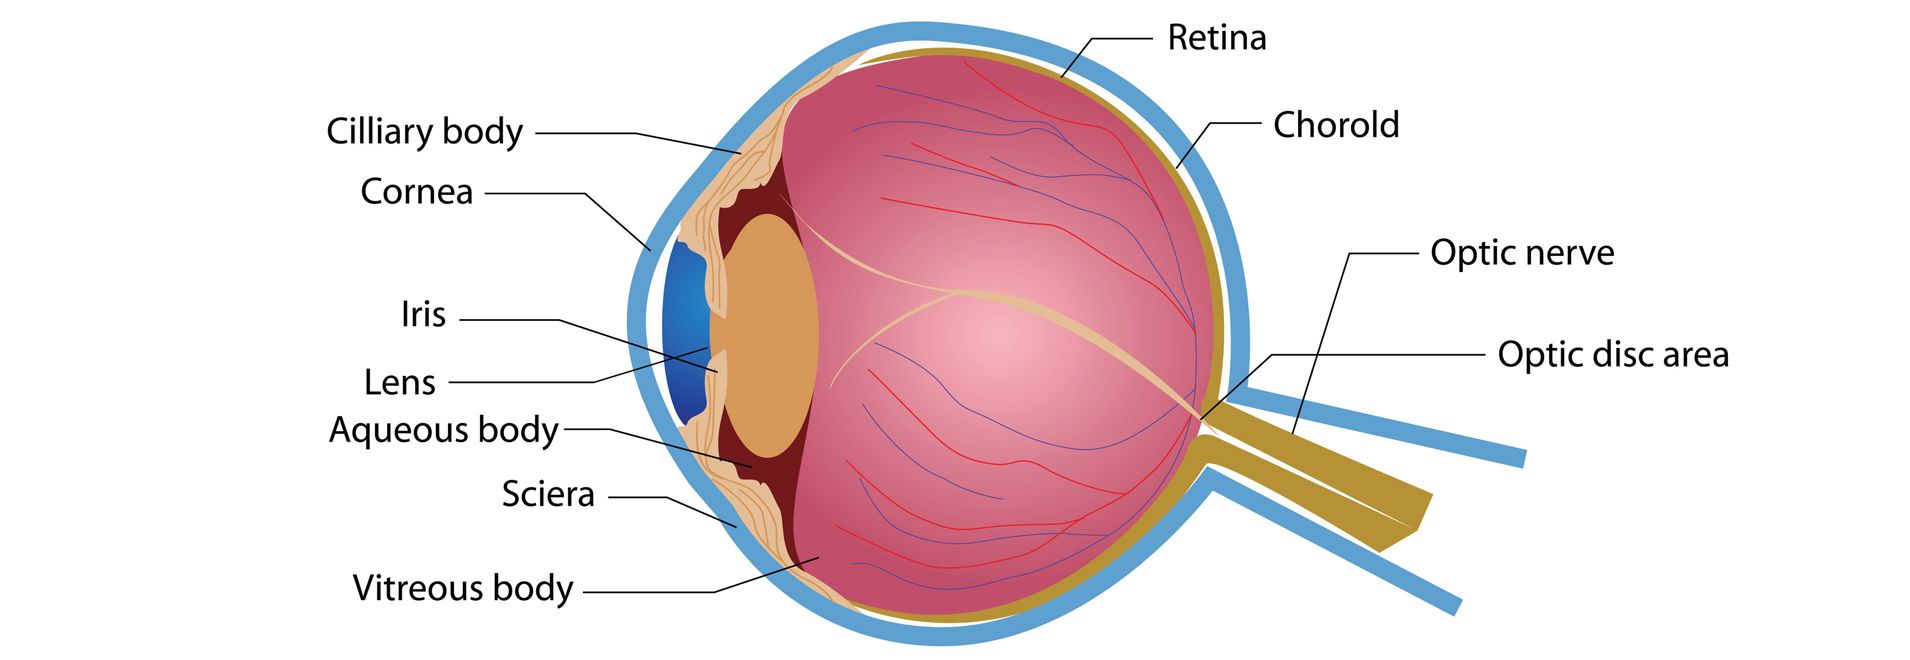
\includegraphics[width=0.8\textwidth]{./images/anatomy-of-the-eye.jpg}
    \caption{Anatomy of the Eye \cite{eyeanatomy-pic}}
    \label{fig:eye-anatomy}
\end{figure}

The scope of this report is limited to the posterior segment of the eyeball as the membranes that are present in it have significant clinical value to ophthalmologists in the analysis and diagnosis of different type of diseases, like myopia and other other ocular diseases \cite{Ronchetti2017}. In particular, we will be focused in the vitreous body, retina, choroid and sclera as they will form integral part of the set of annotations developed for our research in the field of machine learning. 

The vitreous body is an structure characterized by a colorless and transparent gel, mainly composed by water and other aminoacids, proteins, salts and acids. It's located between the lens and the retina and occupies 4/5 of the total volume of the eye and serves mainly to transmit light from the lens to the retina and it's believed that it contributes to the convergence power of the eye \cite{snell1998}. 

Once the light has traveled through the vitreous body, it reaches the retina which is a tissue layer envolving the vitreous. As a part of the central nervous system, the retina "converts the graded electrical activity of photoreceptors into action potentials that travel to the brain via axons in the optic nerve" \cite{purves2001}. In other terms, it converts light into electric signals that are sent to the brain and are interpreted as images.

Supporting the retinal function, between the retina and sclera, the choroid irrigates the outer retina with oxigen due to it's vascular structure through an intrincated layer of capillaries which are connected to arteries via the choroid's vessel layer \cite{snell1998}\cite{choroidExpl}. Several studies \cite{ronchetti2019}\cite{Ronchetti2018} indicate that choroidal thickness has a positive correlation with the development of myopia, which is part of the motivation of this work. 

Finally, the sclera protects the inner part of the ocular globe due to its collagenous structure. Together with the cornea, it serves to contain the internal pressure of the eye and also to contain the forces created by the external muscles of the eye during eye movement \cite{Meek2008}.

\section{Technical Background}\label{TechBack}


\subsection{OCT}
Optical Coherence Tomography (OCT) is the standard technique for producing accurate visualizations of ophthalmic medical images \cite{Garrido2014}. Since OCT scan uses near-infrared low-coherence light waves to produce measurements of the reflectivity vs depth also known as A-Scans\cite{Garrido2014} there is no need for using invasive procedures to extract information from the ocular globe structure. Several A-Scans from consecutive zones can be combined in order to form a 2D image of the posterior segment of the eye where the vitreous, retina, choroid and sclera can be clearly located. Finally, a contiguous set of B-Scans produces a volumetric image that ophtalmologist can use to first evaluate the retinal and choroidal structure and second calculate the layers thickness and issue diagnoses on several type of diseases including various ocular diseases \cite{ronchetti2019}, Diabetes \cite{Jiang2018}, Alzheimer, Glaucoma and other neurodegenerative diseases \cite{DENHAAN2017162}.   

\begin{figure}[H]
    \centering
    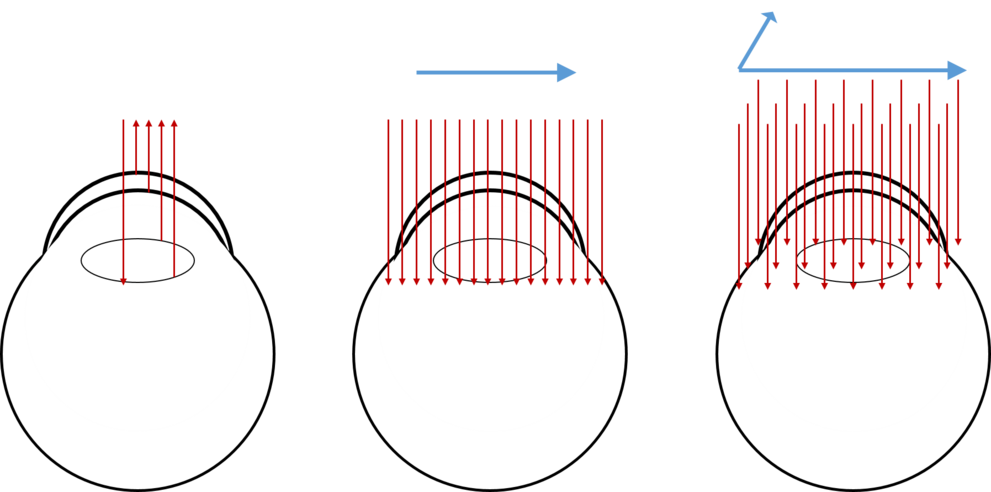
\includegraphics[width=0.4\textwidth]{./images/csm_ABC_scans.png}
    \caption{Scan Types in Optical Coherence Tomography \cite{Willdeman2016}}
    \label{fig:mb-oct-abcscans}
\end{figure}

As stated in the motivation of this thesis, cretinal and choroidal thickness can be measured from OCT scans with the help annotated ground truths establishing the locations of the membranes' boundaries. In the case of the retina, the Internal Limiting Membrane (ILM) divides it from Vitreous on the upper boundary \cite{MACNAIR2015343}, while the Bruchs Membrane (BM) divides the retina from the choroid \cite{BOOIJ20101} serving as the retina's bottom boundary. Subsequently, the Choroidal-Scleral Interface separates the choroid from the sclera \cite{Ronchetti2018}. The mentioned boundaries create a segmentation map within OCT B-Scans where the Vitreous Body, Retina, Choroid and Sclera can be analysed as presented in figure \ref{fig:annotated-oct-scan}. 

\begin{figure}[H]
    \centering
    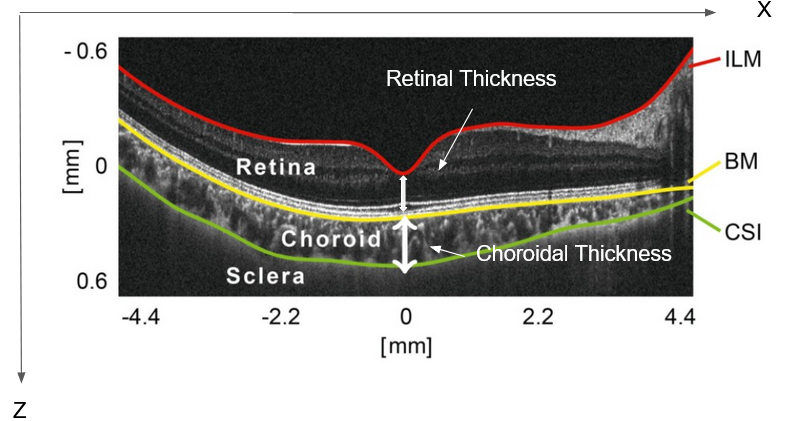
\includegraphics[width=0.8\textwidth]{./images/OCT-Scan.png}
    \caption{Annotated OCT Scan \cite{ronchetti2019}}
    \label{fig:annotated-oct-scan}
\end{figure}

\subsection{Convolutional Neural Networks}

A Convolutional Neural Network (CNNs) is a powerful family of Neural Networks inspired by biological processes and containing Convolutional Layers, used in the field of Deep Leaning. The connection pattern of its neurons is inspired by the visual cortex of animals. Modern CNNs are effective in obtaining accurate models, requiring fewer parameters than fully connected architectures, and are often more computationally efficient because convolutions are easily parallelized on GPU cores.\cite{DIDLBook} CNN-based architectures are common in the computer vision field, as they are prized for their efficiency. 

To be functional, Convolutional Networks need some operations, here we will see the basic and most important ones, the Convolutional Layer itself, padding and stride, pooling layers the use of channels at each layer and the architecture of the modern CNN.

In the case where one wishes to process datasets by collecting and annotating pixels of images one can quickly end up with a network having huge dimensions leading to poor GPU performance, for this reason CNNs are used for data that is not tabular (data consisting of rows corresponding to examples and columns corresponding to features).\cite{DIDLBook} The main role of the CNN is to facilitate the processing of images by reducing them to a form that is easier to examine without losing the features that are essential in the obtaining of a good prediction.


An important concept of CNN is spatial invariance, which means that object recognition is not sensitive to their position in the image. In computer vision, adding convolution to the neural network allows the addition of an inductive visual prior whereby objects can appear anywhere.  Sharing the weights over the location of the object greatly reduces the parameters to be learned, the convolution is moved if the object is moved.\cite{CNNSpatialLocation} The earlies layers of our network should be implementing translation invariance, meaning that it should respond similarly  regardless of where the objects appears in the image. And they should focus on local regions (locality principe) without regard for the contents of the image in distant regions. \cite{DIDLBook}

The translation invariance implies that a shift in the input \(x\) should lead to a shift in the hidden representation \(H\) (represented as matrices in mathematics and as two-dimensional tensors in code). 
This is a convolution as the weighting pixels at \((i + a, j + b)\) in the vicinity of location
\((i, j)\) with coefficients \([V]_{a,b}\) to obtain the value \([H]_{i,j}\) .: 
\[[H]_{i,j} = u + \sum_a\sum_b[V]_{a,b}[X]_{i+a,j+b}\]
Note that both X and H have the same shape and \([X]_{i,j}\) and \([H]_{i,j}\) denote the pixel at location \((i, j)\) in the input image and hidden representation. The translation invariance is only possible if V and u do not depend on \((i, j)\). \cite{DIDLBook}
As described above, in the locality principle , it should no not be necessary to look far away from the location \((i, j)\) to retrives informations to describe what happends in \([H]_{i,j}\), outside a certain range \(|a| > \Delta \: or \: |b| > \Delta\), we should set  \([V]_{a,b} = 0\). And rewrite \([H]_{i,j}\) as follow \cite{DIDLBook}:
\[[H]_{i,j} = u + \sum_{a=-\Delta}^{\Delta}\sum_{b=-\Delta}^{\Delta}[V]_{a,b}[X]_{i+a,j+b}\]



\subsection{U-NET}


\section{Previous work}\label{prevWork}
\subsection{Computer vision methods for detection of early choroidal thickness changes in myopic Asian school children}

\section{Discussion}\label{Discussion}

\subsection{Data Collection}
\subsection{Data Preparation}
\subsubsection{Mask segmentation}
\subsection{Model Development}
\subsection{Model Training}
\subsection{Model Evaluation}

\section{Results}\label{Results}


\newpage
\section{Conclusion}


\section{Future Work}

\markboth{}{}

\newpage

\bibliographystyle{plain} % We choose the "plain" reference style
\bibliography{bibli} % Entries are in the "bibi.bib" file




\newpage
\thispagestyle{empty}
\markboth{}{}
  \normalsize
\begin{center}
\huge{\textbf{ Declaration of Independence}}\\[40mm]
\end{center}
\large
We confirm that the above work has been produced by the authors without any unauthorized assistance and without the use of any other means than those indicated, and that I have marked as such all passages that have been taken literally or meaningfully from published or unpublished writings.\\[50mm]
Bienne, the \today

\newpage



\end{document}